\chapter{Review on needle insertion}

This chapter presents an overview over the research contribution in the field of percutaneous procedures.
Firstly, it will discuss on the action of inserting a needle into tissues, presenting how the interaction forces could be modelled, how the needle reacts, what feedback is required for the procedure and how those information has been combined in literature to achieve some goals like obstacle avoidance or force minimization. Secondly, it will present some robotics solutions designed for assisting a physician with the needle insertion procedure in clinical cases. Lastly will be discussed teleoperation approaches to needle insertion.

\section{Needle insertion model }
Knowledge of interactive forces during needle insertion plays an important role for a precise execution of the procedure. Autonomous system could became able to identify different tissue types, provide a feedback and reduce tissue deformation or needle deflection.
In percutaneous therapy the needle passes through different tissue layers such as skin, muscle, fat and connective tissue. Each layer requires a different amount of force, which varies from patient to patient even for the same tissue type due to prior treatments, age, gender and body mass \cite{Maurin2004}.

Working with a model potentially able to identify the force peak, latency in force changes and separation of different forces such as stiffness and damping with a magnitude that matches the actual measurements is highly desirable.

An example of puncturing is shown in \figurename{ \ref{fig:punct_graph}}: where the force profile is exhibit with respect to time during a needle insertion and retraction in a in vivo liver when other anatomical layer have been previously removed \cite{Maurin2004}.
\begin{figure}
	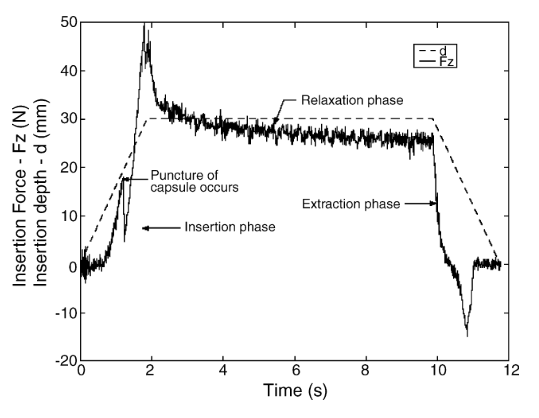
\includegraphics[width=\textwidth]{images/liver_puncturing.png}
	\caption[A needle insertion]{Needle insertion with direct access to the liver  \cite{Maurin2004}}
	\label{fig:punct_graph}
\end{figure}

A model for the puncturing action come from the work of Simone and Okamura \cite{Simone2002}.
They investigated how to model needle insertion forces conducting in vivo experiment with a bovine liver. In their experiments they considered  the puncture of the capsule as the event which divides the insertion into two phases: pre-puncture and post-puncture. In pre-puncture, the force increases steadily and the puncturing event is identified with a sharp drop in the amount of force. In post-puncture, the amount of force vary due to friction, cutting and collision with interior structures.
The authors reports that the total force acting on the needle is
\begin{equation}\label{force_on_needle}
	f_{needle}\left( z \right)  = f_{cutting}\left(  z \right) + f_{friction}\left( z \right) + f_{stiffness}\left( z \right)
\end{equation}
where $z$ is the position of the needle tip.
In \eqref{force_on_needle} the stiffness force is associated to pre-puncture, friction and cutting forces to post-puncture.

\begin{figure}
	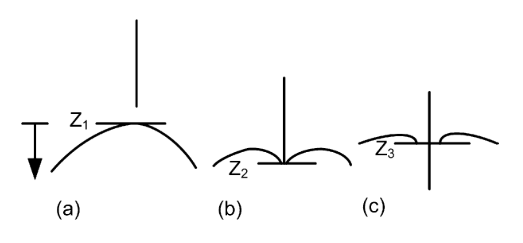
\includegraphics[width=\textwidth]{images/puncture_stage.png}
	\caption[Locations of the tissue surface at each puncturing stage]{Locations of the tissue surface at different stages of needle insertion: (a) pre-puncture, (b) puncture, and (c) post-puncture  \cite{Maurin2004}}
	\label{fig:punct_stage}
\end{figure}

Pre-puncture and post-puncture phases are shown in \figurename{ \ref{fig:punct_stage}}. The stiffness force is due to the elastic properties of the organ and its capsule.
It has been modelled using a non linear spring model:
\begin{equation}
	f_{stiffness} = 	
	\begin{cases}
		0 & z < z_{1} \\
		\alpha_{1}z + \alpha_{2}z^{2} & z_{1} \leq z \leq z_{2} \\
		0 & z > z_{3}
	\end{cases}
	\label{Okamura_stiffnes}
\end{equation}
where $z$ is the needle tip and $z_{1}$, $z_{2}$, $z_{3}$ are respectively pre-puncture. puncture and post puncture position as shown in \figurename{ \ref{fig:punct_stage}}.\\
Friction was modelled with a modified Karnopp model \cite{Dean1985}:
\begin{equation}	
		f_{friction} = 
		\begin{cases}
		C_{n}sgn\left( \dot{z}\right)  + b_{n}\dot{z} & \dot{z} \leq -\Delta v/2\\
		\max\left(D_{n},F_{a}\right) & -\Delta v/2 < \dot{z} \leq 0 \\
		\min\left( D_{p},F_{a}\right) & 0 < \dot{z} < \Delta v/2 \\
		C_{p}sgn\left(\dot{z} \right)  & \dot{z} \geq \Delta v/2
	\end{cases}
	\label{Okamura_friction}
\end{equation}
where $C_{n}$ and $C_{p}$ are negative and positive dynamic friction coefficients, $b_{n}$ and $b_{p}$ damping coefficients, $D_{n}$ and $D_{p}$ static friction values, $\dot{z}$ the relative velocity between needle and tissue, $\Delta v/2$ a minimum threshold on velocity and $F_{a}$ is the sum of non frictional forces applied to the system.\\
The cutting force was modelled as a constant $\alpha$ for a given tissue:
\begin{equation}
	\label{Okamura_cutting}
	f_{cutting} = 	
\begin{cases}
	0 & z_{tip} \leq z_{2}, t<t_{p} \\
	\alpha & z_{tip} > z_{2}, t\geq t_{p} \\
\end{cases}
\end{equation}
where $z,z_{1},z_{2}$ are the same that appears in \eqref{Okamura_friction}, $t$ is time and $t_{p}$ the puncturing time.

The same authors also investigated the effect of needle diameters and tip type on insertion forces \cite{Okamura2004}.
They found a correlation between the tip type and insertion forces: they notice that the forces increases as the needle tip type change from triangular to bevel, and from bevel to cone.
A bevel angle does not affect the axial force significantly but for each of the tip types, the increase of the needle diameter increases the insertion force.
\begin{figure}
	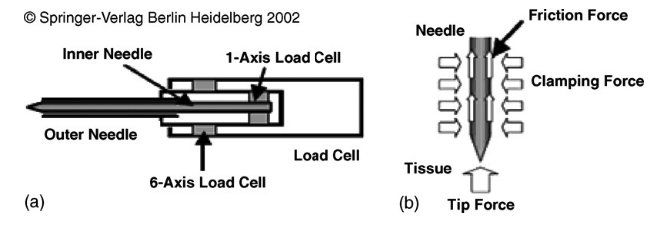
\includegraphics[width=\textwidth]{images/Kataoka.png}
	\caption[The seven-axis load cell]{(a) Structure of the seven-axis load cell and (b) the forces acting on a needle inside the tissue \cite{Kataoka2002}}
	\label{fig:kataoka_load_cell}
\end{figure}

Another work is the one by Kataoka \textit{et al.} \cite{Kataoka2002}: using a specially developed seven-axis load cell for measuring and separating forces during needle insertion, they performed experiments on an exposed prostate of a defrosted beagle cadaver.
They were able to measure three different forces acting independently  of the needle: the tip force, the friction force and the clamping force.
In \figurename{ \ref{fig:kataoka_load_cell}} both custom load cell and these forces acting on needle  are shown.
The tip force, that acts on the needle in the axial direction, was assumed to be primarily related to cutting; the authors report that the shape of the tip affects the magnitude of this force.
The Friction force, that acts on the sidewall of the needle shaft in axial direction, was considered to be the sum of Coulomb and viscous frictions.
The clamping force, which acts on the sidewall of the needle shaft in the normal direction, has been explained as the resistance force performed by the tissue due to its compression away from the needle path.
The clamping force increases as the needle is inserted into the tissue and its magnitude is affected by the needle gauge and the incision shape.
After the puncture, the tip force decreases immediately reaching the value of the cutting force, which is a constant.
This decrease occurs because the prostate capsule acts like harder layer on top the inner tissue.
%However, generalizing constant cutting force for all tissue types may not be sufficiently accurate.
On the contrary, the friction increases proportionally to the true insertion depth according to the needle diameter.
The total axial force is the sum of the tip force and the friction force, with the contribution coming from clamping force included in the friction force value.
The authors calculate the insertion depth subtracting the surface motion (indentation) from the driving distance of the needle neglecting the fact that tissue surface, after deformation and compression in the penetration phase, tends to slide back on the needle after puncture. This could be a source of inaccuracy.

Matsumiya \textit{et al.} \cite{10.1007/978-3-540-39899-8_34} presented an experimental study of robotic needle insertion into a formaldehyde-fixed (FA- fixed) human vertebra and measured forces and torques during the insertion.
They used a needle with triangular pyramid tip and a robot developed for percutaneous vertebroplasty, which could insert the needle with bidirectional axial rotation.
Their work showed a strong correlation between the axial
force variation during insertion and the distribution of the bone local CT-value along the needle path.
A remarkable factor of their result is that the axial force during robotic insertion into human femoral head was found to be smaller than that during manual insertion (about 1/3 of the manual insertion).
They accounted two reasons for that: first, the robot can hold the needle in a more stable manner than human during the insertion, second, the  speed and angle of rotation can be varied more easily in a robotic insertion.
\begin{figure}
	\centering
	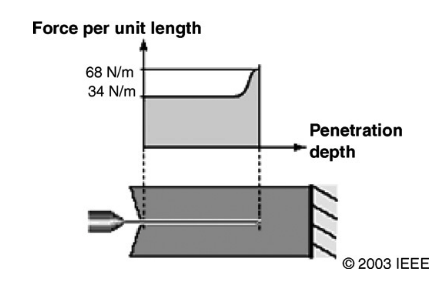
\includegraphics[width=(\textwidth/2)]{images/DiMaio_force_distribution.png}
	\caption[Force distribution in puncturing]{Estimated needle force distribution (insertion velocity is 1 mm/s). This distribution is taken from the estimated tissue phantom forces at nodes along the needle shaft  \cite{DiMaio2003}}
	\label{fig:DiMaio_force_distribution}
\end{figure}

DiMaio and Salcudean in \cite{DiMaio2003} and \cite{DiMaio2005} explored the relationship between needle force and 2D tissue deformation using a planar robot, an artificial tissue phantom and a CCD camera. The force distribution along the needle shaft, shown in \figurename{ \ref{fig:DiMaio_force_distribution}}, indicates the existence of two forces: an axial friction force, uniform along the shaft, acting between needle and tissue, and a force placed at needle tip, which results from the cutting of the tissue and is approximately twice the friction force \cite{DiMaio2003}.
During penetration, the shaft force increases with insertion velocity while the force peak at the distal end of the needle appears to be independent of velocity, becoming less prominent at higher velocities.

The results of all the above studies agree with the model presented by Simone and Okamura \cite{Okamura2004}.

\section{Needle deflection}
The problem of needle deflection is one of the reasons for inaccuracy in needle insertion procedures. During the insertion phase, the tissue around the needle tip is compressed and, due to the needle geometry, the unbalanced resistance of the forces against the compression can deflect the needle \cite{katakoa2001}.
	\begin{figure}
	\centering
		\subfloat[A symmetric-tip needle exerts forces on the tissue equally in all directions, so cutting the tissue occurs in the moving direction of the needle tip]{
			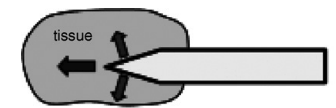
\includegraphics[width=\textwidth/2 ] {images/simmetric_needle_tip.png}
			\label{fig:simmetric_needle_tip}}
	\hspace{0.5cm}
		\subfloat[A bevel-tip needle exerts forces asymmetrically so cutting the tissue occurs at an offset angle depending on the bevel angle, needle flexibility and tissue properties.]{
			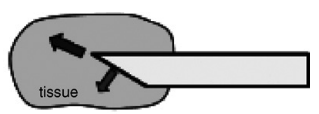
\includegraphics[width=\textwidth/2] {images/bevel_needle_tip.png}
			\label{fig:bevel_needle_tip.}}
		\caption[Forces exerted with different needle shape]{Forces exerted with different needle shape \cite{katakoa2001}}
\end{figure}
The previously addressed work by Okamura \textit{et al.} \cite{Okamura2004}, presents also the effect of needle geometry on needle bending.
They found that needles with smaller diameters and bevelled tips lead to more needle bending, whereas conical and triangular tips manifest less bending. They also noted that “a bevelled tip needle bends because it's asymmetry and receives higher force on one side”.
Another reason for bending in a needle with a symmetric-tip (triangular or conical) could be the changes in the mechanical properties of the material trough which the needle is inserted. Material inconsistency may also be a reason for inconsistent bending of bevelled tip needles.
\begin{figure}
	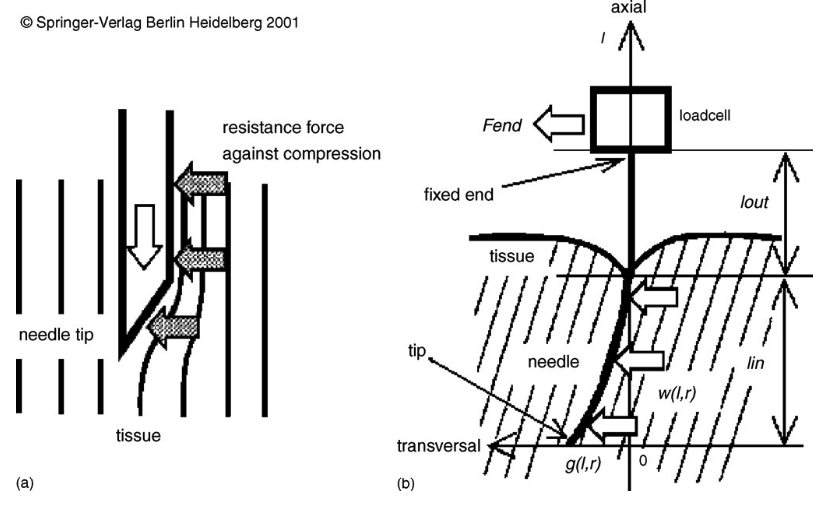
\includegraphics[width=\textwidth]{images/kataoka_model.png}
	\caption[Needle bending model]{A force-deflection model for a bevelled tip needle during penetration into soft tissue: (a) force on a needle tip; (b) force and deflection of a needle \cite{katakoa2001}}
	\label{fig:kataoka_model}
\end{figure}

A model for the force-deflection of a bevelled tip needle during insertion has been proposed from Kataoka \textit{et al.} in \cite{katakoa2001}.
A physical quantity called \textit{infinitesimal force per unit length} was used in order to find the amount of needle deflection during insertion.
This quantity was adopted from the traction definition \[\lim_{\Delta l \rightarrow0}\left(  \dfrac{\Delta F_{s}}{\Delta l}\right) \] where $\Delta F$ is the force acting on the segment of a deflected needle and $\Delta l$ is the length of a deflected needle segment.\\
According to the model, which is shown in \figurename{ \ref{fig:kataoka_model}}, the needle deflection is described as
\begin{multline}
		g\left( l,r \right)  = \dfrac{W\left( r \right) }{24EI} \left( l^{4} -4l_{in}\left( l^{2}_{in} + 3L_{in} l_{out} +3l^{2}_{out}\right)l\right.  \\\left.  + l_{in} \left( 3l^{3}_{in} + 12l^{2}_{in}l_{out} + 18l_{in}l^{2}_{out} + 8l^{3}_{out} \right) \right), \quad 0 \leq l \leq l_{in}
		\label{Eq:Neddle_deflection}
\end{multline}
where $l$ is the length of the needle, $l_{in}$ and $l_{out}$ the lengths of the needle inside and outside the tissue, respectively, $W(r)$ the force per unit length, $r$ the needle radius, $E$ Young’s modulus for the needle (2.0×10^{2} GPa for stainless steel material) and $I$ is the moment of inertia of the needle.
They considered $W(r)$ to be constant for needles with the same diameter.

The experiments, performed into a swine’s hip muscle tissue, measured the needle deflection using X-ray imaging. They compared the amount of the measured deflection with the deflection predicted by \eqref{Eq:Neddle_deflection}. The results shows that the slope of displacement versus the length at different needle diameters was comparable; however, the predicted deflection was smaller than the measured one.
The authors suggested that there is another degree of freedom, a moment or a rotational component, which accounts for the actual deflection. In their model, the mechanical properties of soft tissue, tissue deformation and the bevel angle of the needle are not considered. It cannot be generalized from their results whether, in insertions with the same needle into different tissues, the value of $W$ would still remain the same.

Webster \textit{et al.} performed needle insertion into a rubber-like simulated muscle using needles with different bevel angles \cite{WebsterIII2005}.
From their result decreasing the bevel angle increases the amount of needle deflection, but the bevel angle has little impact on the amount of the axial force.
They also performed insertion with different velocities founding that the velocity of needle insertion in homogeneous, relatively stiff phantom tissue had no discernable effect on the amount of needle deflection. Velocity has an impact on the amount of the axial force.
While the result of their study on needle deflection matches with in vivo observations, the velocity ones lacks of an in vivo validation.

\section{Feedback during procedures}\label{Feedback_during_procedures}
Other causes of inaccuracy in percutaneous therapy are: physiological changes that occurs in the organ between the planning and treatment phases, glandular swelling during the operation, difference in tissue types involved in each procedure, differences in mechanical properties of healthy and diseased tissue, changes of mechanical properties when a tissue is damaged and variability of soft tissue properties for the same organ in different patients.\\
Medical imaging (CT-scan, ultrasound, fluoroscopy, MRI)
plays an important role in image-guided procedures whose rely on powerful computer systems for navigating, planning, tracking and modelling.\\
From several studies and clinical practices, it is known that offline medical imaging does not provide enough accuracy for precise procedures. Therefore, real-time imaging techniques have been developed \cite{Peters2001}.\\
There are basically two approaches that are compatible with a conventional surgical procedure because absence of/ very limited consequences on the surgeon:
\begin{description}
	\item[MRI] MR imagers to be used over surgical procedure. Special machine has been designed to improve access to the patient and/or  allow the use of standard surgical tools and instrument in close proximity to the scanner.
	\item[US] Ultrasound is the other wide used interventional imaging modality. However it has inferior image quality than the one attainable from even low-field intra-operative MRI. 
\end{description}
Many works in literature explore the mapping between pre operative imaging data and intra operative US images because of the expense of intra-operative MRI equipment.
One of the requirements for precise control of (robotic) needle insertion is the capability to identify tissue types and their deformation in real time.
There are two main feedback involved in needle insertion procedures: visual  and tactile feedback. The former provide information on tissue type, obstacles and needle path between tissue, the latter provide information about the puncture moment \cite{Abolhassani2007}.
An evaluation on the effects of visual and haptic feedback comes from the work of Gerovichev \textit{et al.} \cite{Gerovichev2002}. Using a virtual needle insertion simulator, they studied the detection of puncture of a layer with two groups of volunteers.
One group had medium exposure to a haptic interface and the virtual environment and low expertise to real needle insertion and the other group had extensive experience in real needle insertion without having previous experience with haptics.
The results of this study show that the addition of force feedback reduces the error in detection of transitions between tissue layers; however, real-time visual feedback provides greater improvements in performance than force feedback.
With robotic applications in mind, the work from Washio and Chinzei \cite{Washio2004} carried out manual and robotic needle insertion experiments into bovine liver founding that a force sensor could detect the moment of puncture slightly faster than video-based detection. In addition, they found that a force sensor could be more sensitive than a skilled surgeon for detecting the moment of puncture.

Finally the work by Mathiassen, Dall'Alba \textit{et al.} \cite{Mathiassen2013} provide an improved solution for the problem of real-time tracking of a needle inside a tissue using an ultrasound probe. This methodology is valuable because it could be also used in conjunction with a robotic platform.
\section{Needle insertion techniques}
Some researches, like Alterovitz \cite{Alterovitz2005} and Di Maio \cite{DiMaio2003Steering} have studied the flexibility of the needle to increase manoeuvrability. They refer to this technique as needle steering.\\
Other solutions applied the same principle to define trajectories with the aim of reducing needle deflection and tissue deformation.\\
Upon the model presented in \cite{DiMaio2003}, DiMaio and Salcudean carried out a study on the kinematics of motion-planning: they introduced the concept of \textit{needle manipulation Jacobian} for needle steering and manipulation.
The Jacobian  is defined as the relationship between the needle tip and the base velocities
\begin{figure}
	\centering
	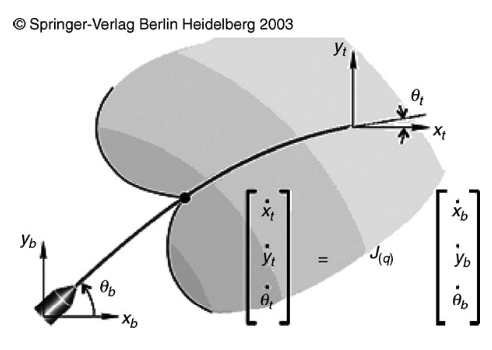
\includegraphics[width=\textwidth/2]{images/needle_Jacobian.png}
	\caption[Needle manipulator Jacobian]{Steering and the needle manipulation Jacobian \cite{DiMaio2003}}
	\label{fig:needle_jacobian}
\end{figure}
\begin{equation}
	J = 
	\left[ 
	\begin{matrix}
		\dfrac{\partial x_{t}}{\partial x_{b}} \qquad & \dfrac{\partial x_{t}}{\partial y_{b}}  \qquad &\dfrac{\partial x_{t}}{\partial \theta_{b}} \\ \\
		\dfrac{\partial x_{t}}{\partial y_{b}}  \qquad& \dfrac{\partial y_{t}}{\partial y_{b}}  \qquad& \dfrac{\partial y_{t}}{\partial \theta_{b}} \\ \\
		\dfrac{\partial \theta_{t}}{\partial x_{b}}  \qquad& \dfrac{\partial \theta_{t}}{\partial y_{b}}  \qquad & \dfrac{\partial \theta_{t}}{\partial \theta_{b}}
	\end{matrix}
	\right]^{T}.
\end{equation}
An illustration could be found in \figurename{ \ref{fig:needle_jacobian}}.\\
In order to plan the needle trajectory, they incorporated into the model soft tissue motion, needle flexibility and a physically based contact. To avoid the obstacles they act on the base, outside the tissue. The steering involved on the needle moves the tissues around it in such a way that the obstacles on the path are avoided. This is done using a task space potential field approach. The proposed methodology has been validated via simulation and robot-controlled trajectory experiments in a transparent PVC phantom.\\

Similar to the steering technique of DiMaio and Salcudean, but with a simplified model for the tissue and for the flexible needle, is the one by Glozman and Shoham \cite{Glozman2006}.
They performed a fast path planning with real-time needle tracking in order to avoid an obstacle and hit a target.
Their model approximate the tissue with virtual springs, furthermore they use an inverse kinematic approach to translate and orient the needle base.\\
This work carries out that the needle base trajectory can be varied and can be optimized to minimize the lateral pressure of the needle shaft on the tissue especially if the operation is robot assisted: in fact they were able to decreased both the base stroke and the pressure by relaxing the tip orientation requirement of being tangent to the path.

Reducing insertion forces while achieving less tissue deformation and needle deflection is a wide investigated topic and many insertion techniques have been proposed end tested.
 
Meiklejohn \cite{MEIKLEJOHN1987} showed that rotation of an epidural needle significantly decreases the force required to puncture the dura. However, it was recommended that rotation should be applied only during the initial part of needle insertion because after reached the epidural space, there is a likelihood of tearing the dura due to the bevelled shape of the needle tip.

Hochman and Friedman\cite{MEIKLEJOHN1987} studied the effect of different manual needle insertions on the force necessary to puncture and advance a needle through tissue phantoms for applications in dentistry. They exploited both a linear insertion technique and a bidirectional rotation–insertion technique on tissue phantoms with different densities and using needles of different gauges. The bidirectional rotation–insertion technique involves insertion while rotating the needle through 180° in each direction about its axis. Their results revealed that bidirectional insertion requires less force for puncturing and penetration than linear insertion irrespective of the material and needle gauge.
Little if any deflection was observed when bidirectional rotation was used in an insertion with a bevel-tip needle. 
%%TODO Chiedere a Riccardo cosa ha capito
The study on the effect of different trajectories on tissue indentation and friction force come from two works from Abolhassani \textit{et al.} \cite{AbolhassaniRoboticsNeedle2004}\cite{Abolhassani2004}.
They performed experiments on ex vivo turkey tissue with its skin intact using a 6-DoF force/torque sensor and a robot with two degrees of freedom: translation in the horizontal direction and rotation about the translational axis.\\
A needle with a bevel tip was used for the experiments and the same upward orientation of the bevel tip at the skin contact point was considered. For each insertion at the same, constant, velocity, they evaluate the effect of different rotational motions. The following has been considered: no rotation, continuous rotation with different speeds, bidirectional rotation with different rotational angles and speeds and needle rotation based on forces orthogonal to the insertion direction.\\
They were able to show that with a rotational motion they can reduce the amount of tissue indentation as well as the friction force between the needle shaft and the tissue.
The lateral forces are the result of forces exerted by the tissue on the needle which are also the cause for the needle deflection. By controlling the rotational motion, keeping as close to zero as possible the lateral forces acting on the needle, they obtained the best result among different types of rotational motions.
In general, physicians tend not to favour needle rotation although it reduces friction forces and makes the insertion procedure easier. The main reason for this choice is the increased trauma to the patient in the region of penetration when exceeding in rotations. In their study, Abolhassani \textit{et al.} also tried different types of translational motions for needle insertion showing that an increase in needle insertion velocity could reduce the amount of tissue deformation.

\section{Robots for needle insertion}
With the intention of increasing precision, reducing procedure duration, especially when multiple insertion are needed, and achieve a better control on phenomena like needle bending and tissue deformation, robots have been introduced to assist surgeons.
\subsection{The first medical robot}
Biopsy in neurosurgery can be accounted as the first medical technique to benefit from the support of robotics: in 1985 the UNIMATION PUMA 200 has been placed into a neurosurgical operating room for the purpose of holding and manipulating a biopsy cannulae \cite{Kwoh1988}.
The official publication came a few year later in 1988, and explained the procedure involved: the Stereotactic brain surgery as technique for guiding the probe, augmented with a 3D localization system provided with a CT scanner.

The advantage of a robotic assisted Stereotactic procedure lies in a faster, more automated, flexible, reliable and accurate procedure. It could be used for both the body and the head, and can be fully integrated with the CT scanner.
In fact, previously, for each probe insertion, the surgeon should look at the CT scanner, read the scale from the stereotactic frame, adjust the frame according to the computer output and finally drill a hole in skull.%%TODO burr o drill questo è il dilemma
Adjustment between different trajectory settings were almost impossible because the frame had already been draped under sterile condition.

As mentioned in previous sections, there are two main safe techniques that provide real-time image modality during clinical procedures: MRI and US.
Robotic equipment has to deal with that, especially with MRI due to the high magnetic field.
The first medical robots were an adaptation of industrial models of those times. Later researchers focus they attention on building machines more thigh to medical application. Improvements regard materials, placements and integration with the procedure the robot was build for.
\subsection{MRI compatible robots for needle insertion}
A manipulator operating in MRI must satisfy the following conditions:
\begin{enumerate}
	\item safety even under malfunction or accidents, e.g., a power failure
	\item no artefacts or distortions on the image caused by the installed robot in the scanner
	\item size small enough to be fixed on the bed of the scanner or to be installed nearby.
\end{enumerate}
The work of Kwoh \textit{et al.} \cite{Kwoh1988}, despite the integration with CT-scanner, requires the patient to be pulled in and out the scanner every time a new image was acquired.
To overcome this limitation, Masamune in \cite{Masamune1995} presents a robotic Stereotactic frame (\figurename{ \ref{fig:robotic_stereotactic_frame}}) with 6-DoF that could operate under an MRI scanner.
The frame design is similar to the ISEKI-frame developed for manual stereotactic surgery with an arc-style isocentric mechanism chosen for mechanical safety and simplicity. In fact each axes is independently controlled assuring high precision. Furthermore there is no possibility of collision with the patient even if the manipulator is out of control.\\
To be compatible with an MRI scanner this frame has been build mainly with synthetic PET resin, other few parts that should be stronger or very precise are made by non-magnetic steel, brass, aluminium, delrin or ceramic.
Actuation has been provided through ultrasonic motors made of non-magnetic materials whose can move properly in strong magnetic fields.
Further advantages of an ultrasonic motor are its high torque performance and physical rigidity even when the power source is off. Consequently, the manipulator cannot move from its own weight even during a power failure.\\
Another advantage of this device, is that no calibration procedure is needed before scanning.
Despite an accurate material selection and design, the frame causes noise artefacts in MRI images while powering the motors.
Masamune's stereotactic frame needs an MRI-compatible needle.\\
\begin{figure}[h]
	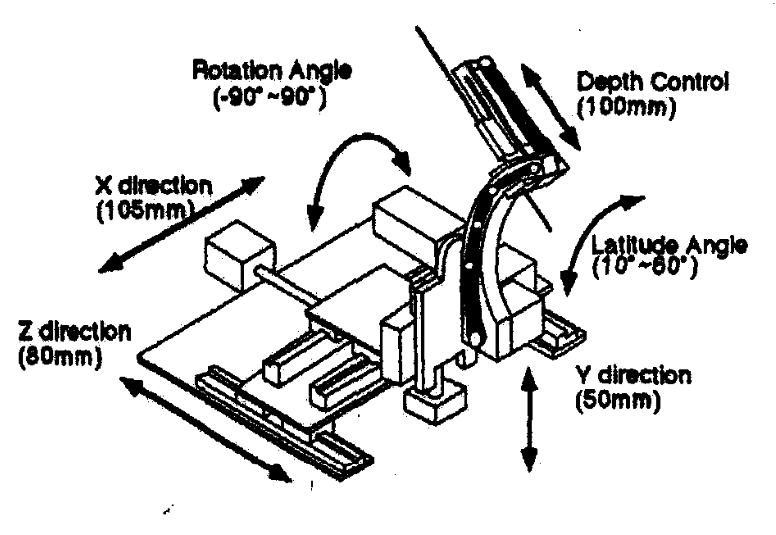
\includegraphics[width=\textwidth]{images/robotic_stereotactic_frame.png}
	\caption[Masamune's stereotactic frame]{Mechanism of the needle insertion manipulator and its range of movement; XYZ axis for positioning, latitude angle and rotation angle for orientation, and depth control for needle insertion \cite{Masamune1995}}
	\label{fig:robotic_stereotactic_frame}
\end{figure}

\begin{figure}[h]
	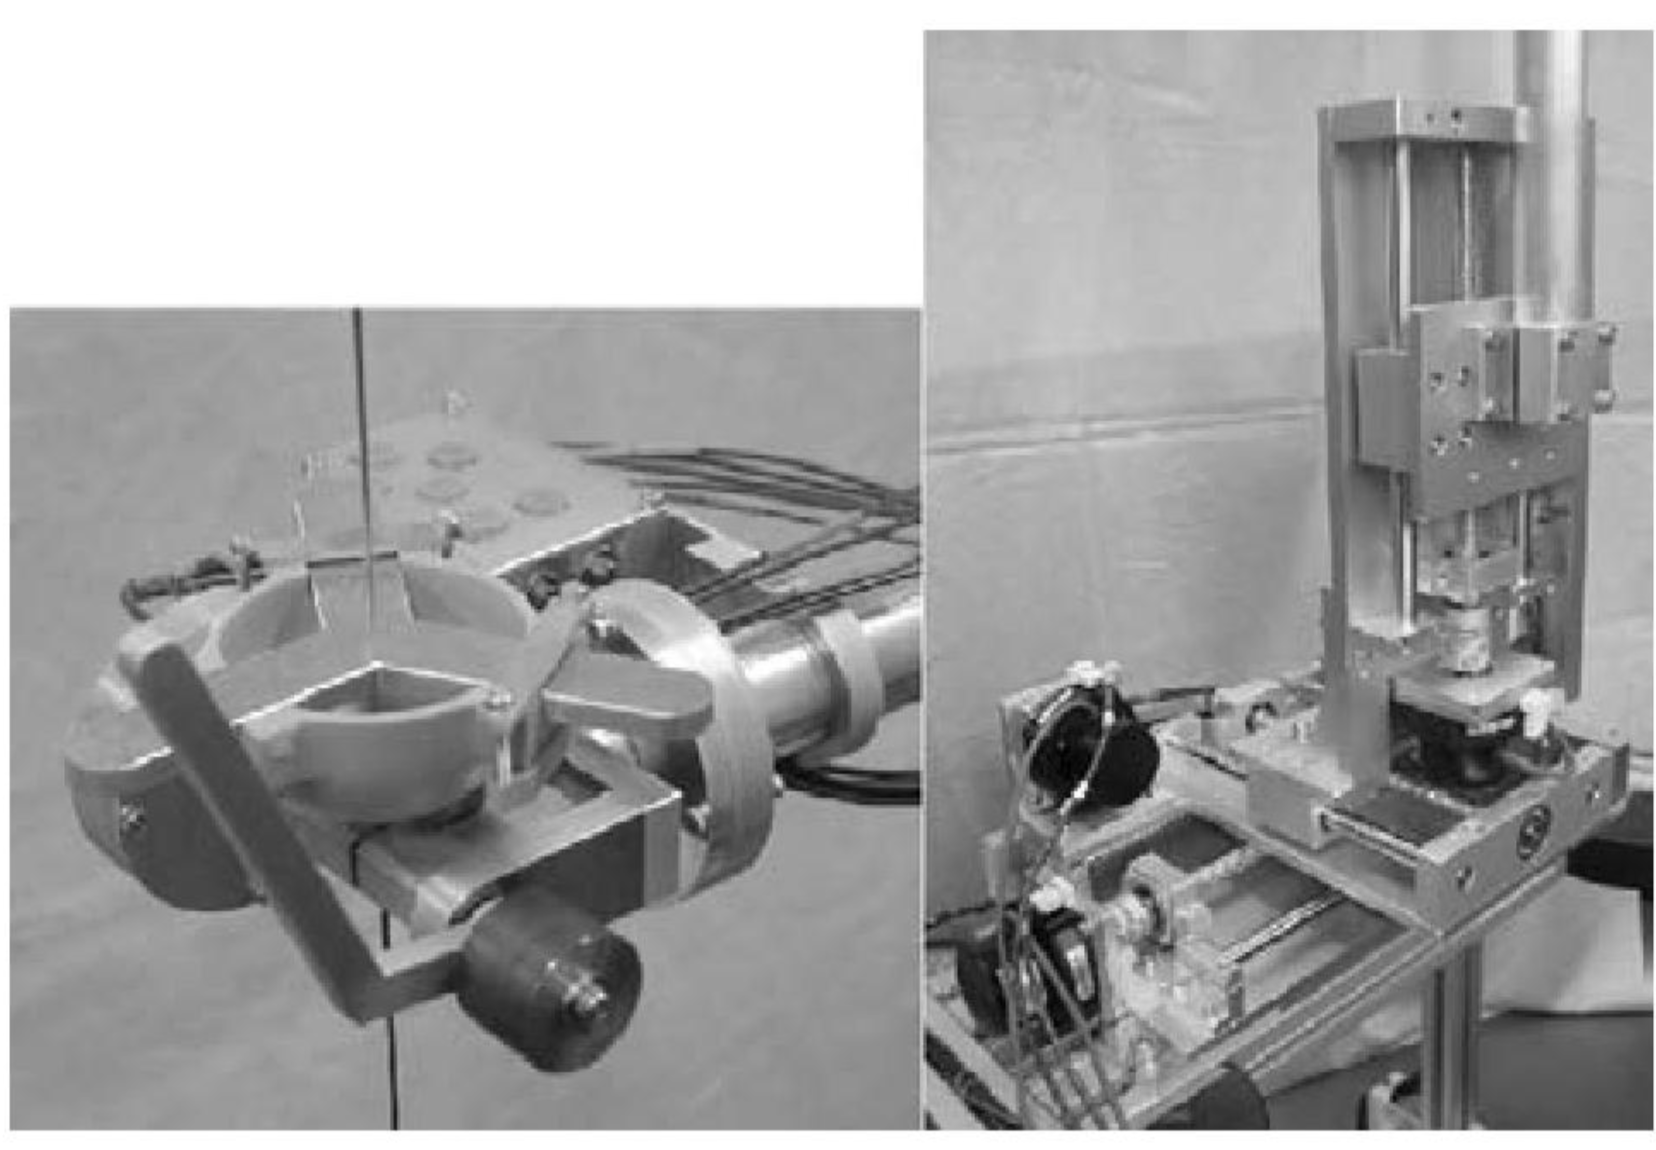
\includegraphics[width=\textwidth]{images/RCM_robot.png}
	\caption[MR compatible robot with RCM]{MR compatible RCM needle guiding robot; Active 3-DoF XYZ stage (right) and Passive 2-DoF end effector (left) \cite{Hata2005}}
	\label{fig:RCM_robot.png}
\end{figure}
Another example of MRI compatible robot is the one developed by Hata \textit{et al.} \cite{Hata2005}.
This robot isn't fully actuated as Masamune's stereotactic frame, but it's partially actuated. It has 3-DoF of translation active with ultrasonic motors and 2DoF of rotation passive and unconstrained. With this selection the surgeon can freely select the needle intersection path while constantly pointing at the pre-defined site. The robot  is installed on the side of the bed, and reaches with its arm the patient's body.
Although with this robot the percutaneous insertion has to be manually performed, it's interesting the use of the Remote Centre of Motion control to assist surgeon in reaching the target.\\
Because of MRI compatibility this robot is made of aluminium and other non magnetic materials and use ultrasonic motors for actuation as done for Masamune's stereotactic frame. The passive 2-DOF end-effector is the part of the robot which could easily cause undesired artefacts on the MR image because it is located near the imaging region. Thus encoder with working principle based on electrical signal are undesirable.
Because of that, non-magnetic optical encoder has been designed and optical fiber has been used to transmit the signal to an external acquisition electronics.
For performing the RMC control, the robot control system has been integrated with an MR imaging system in charge of acquiring images and detecting needle position.
\figurename{ \ref{fig:RCM_robot.png}} shows the robot and its end-effector.

\subsection{US based robots for needle insertion}
The other kind of image guided interventions are US based.\\
A robot for accurate needle insertion driven by a real-time visual servoing to compensate for real-time organ deformation and motion is presented in the work of Hong \textit{et al.} \cite{Hong2004}.
The robot consists of a 5-DoF passive arm to position the needle at the skin entry point and a 2-DoF needle-driving end-effector for automatic needle-insertion control.
A spring buffer has been placed between the active control part and the 5-DoF passive arm to absorb body tremors and maintain a tolerable pressure between probe and skin.\\
The ultrasound probe and the needle driver are interconnected to form a single unit called \text{UMI}. This structure allows the target and needle to be placed on the same image plane so that the operator could observe the relationship between the position of the needle and the target while performing the intervention.
The needle driver uses a friction transmission: a motorized silicon roller increases the friction between the needle and the roller. This solution could be affected by slippage that can be addressed through the visual feedback. The needle access angle can be changed upon the isocentric movement.\\
By using visual servo control, no sensors or markers are needed, furthermore needle bending or slippage can be corrected and controlled through image processing.  Furthermore the system is not sensitive to calibration problems since only vision is used to stabilize the control mechanism.\\
Every parameter required for the UMI control is computed and determined in the image feature space through image processing.
The UMI system determines the orientation and position of the target and the feedback is sent back to the controller to correct the needle path. 
The target position is tracked by a motion-optimized active contour model. Needle recognition is performed using the Hough transform: points on the same line in an image are gathered into one point in parametric space and the most ‘concentrated’ point is related to the dominant line in the image plane, which eventually represents the needle.
After the dominant line is found, this line is used as a guideline to locate the tip of the needle: when a unconnected point with huge gap is detected in the line, it is considered to be the endpoint.
\begin{figure}
	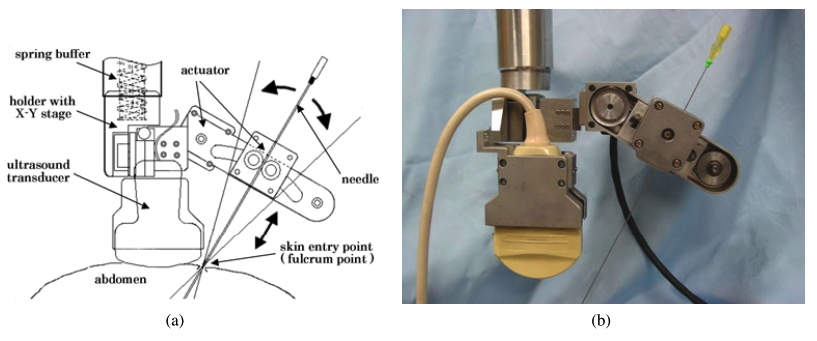
\includegraphics[width=\textwidth]{images/UMI.png}
	\caption[UMI schema]{Ultrasound-guided motion adaptive needle-insertion instrument (UMI). (a) Schematic and (b) appearance. \cite{Hong2004}}
	\label{fig:umi}
\end{figure}

The second example of robot reported in this subsection is the one developed by Balten \textit{et al.} \cite{Balter2017}.
It's a comprehensive platform that incorporate stereo vision, ultrasound and force guidance to build a fully automated venipuncture device.
\begin{figure}
	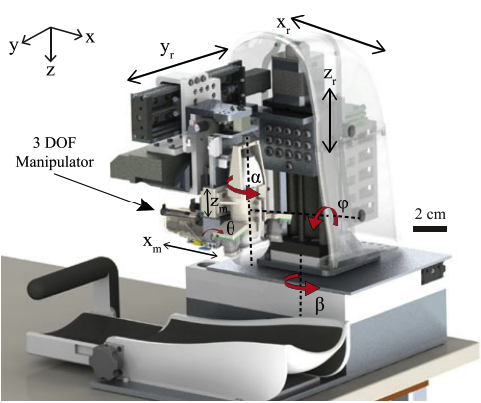
\includegraphics[width=\textwidth]{images/venipuncture_robot.png}
	\caption[The venipunture robot]{Conceptual design of the venipuncture robotic system. \cite{Balter2017}}
	\label{fig:venipuncture_robot}
\end{figure}
The device combines 3D NIR and US imaging, computer vision and image analysis software, and a 9-DoF needle manipulator within a portable shell.\\
The device maps the 3D position of a selected vessel and inserts a needle into the center of the vein with real-time image and force guidance.
NIR, US and needle insertion subsystems are integrated into a compact end-effector that allows each subsystem to remain aligned regardless of the end-effector orientation. A force sensor is also coupled to the motorized needle insertion to obtain the puncturing feedback during the venipuncture.\\
Two separate motion control schemes have been implemented using stereo vision, US, and force measurements to adjust the needle position in real-time.
The device scans the patient’s forearm using the NIR system to create a 3D representation of the vessels and estimate their depth below the skin. 
A puncturing site is selected by the clinician via the graphical user interface, then the US probe is positioned over the site to provide view of the vessel and confirm blood flow, finally the robot orients and inserts the needle.
\begin{figure}
	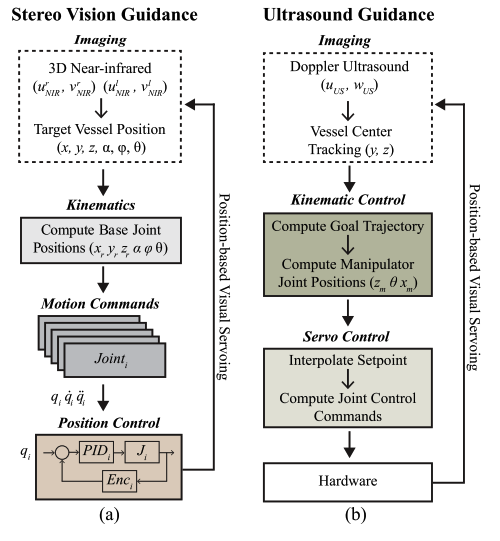
\includegraphics[width=\textwidth]{images/control_scheme_vessel.png}
	\caption[Venipuncture device control schema]{Motion control scheme in which position data is extracted from the image sensors and used to guide robotic motions. (a) Stereo vision- based, and (b) US-based visual servoing. During the venipuncture, the force sensor helps compute the needle tip location, serving as the third method of feedback. \cite{Balter2017}}
	\label{fig:control_scheme_vessel}
\end{figure}
The motion control scheme of the robot is summarized in \figurename{ \ref{fig:control_scheme_vessel}}.
They implemented a position-based visual servoing, as opposed to an image based approach, because this technique is more robust than the image-based visual servoing that takes into account only the error between the current and desired feature on the image plane. By estimating the pose of the target with respect to the camera in a 3D environment, this approach is more robust both to a temporary exit of the needle from the visual field of the probe  and/or to a needle occlusion  in the US images due to noisy acoustic signals.

\section{Teleoperated needle insertion }
In the previous section some example of robots designed for the needle insertion task were presented. All of those are useful help both for the surgeon and patient because  they are deigned for of minimizing errors, times and increasing safety in the procedure. These designs either provides help for needle placement while leaving in charge the expert for the insertion phase, or provide a fully automated procedure with the expert that only select on a remote device the needle target.

A different category of devices is the one where the procedure is performed by an expert acting remotely on the needle. Those system can also provide a feedback on the action performed.
\begin{figure}
	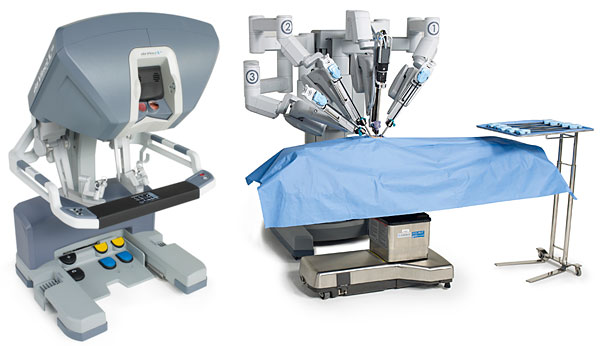
\includegraphics[width=\textwidth]{images/da_vinci.jpg}
	\caption[The Da Vinci Surgical System]{The Da Vinci Surgical System \cite{intuitive}}
	\label{fig:da_vinci}
\end{figure}
In medical procedures the most famous telesurgery robot is the Da Vinci Surgical System shown in \figurename{ \ref{fig:da_vinci}} which is routinely used in the clinic treatments worldwide and has shown to achieve operations levels which are comparable or better than those achievable by human surgeons. The system provide only a 3D visual feedback to the surgeon.
In needle insertion procedure, as discussed in Section \ref{Feedback_during_procedures}, providing an haptic feedback in addition to the visual feedback is desirable to improve procedure's outcome.

\begin{figure}
	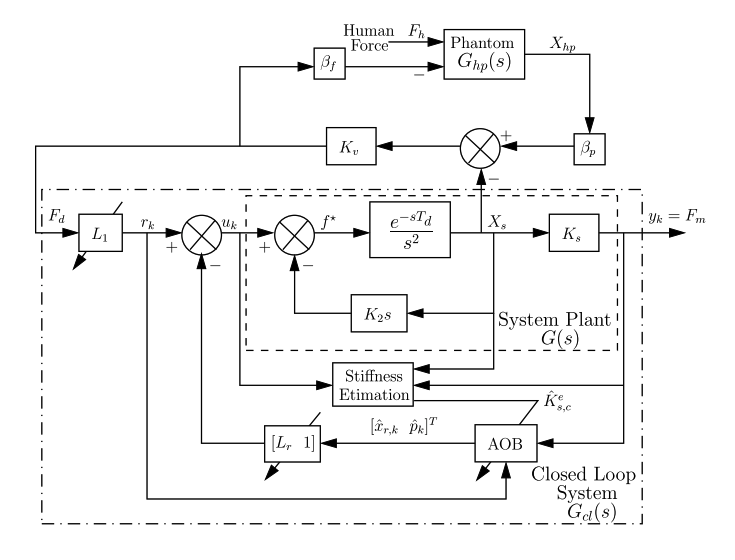
\includegraphics[width=\textwidth]{images/zarrad_scheme.png}
	\caption[Haptic teleoperation schema (Zarrad)]{Teleoperation control scheme for each Cartesian dimension. \cite{Zarrad2007}}
	\label{fig:zarrad_scheme}
\end{figure}

Zarrad, Poignet, Cortesao and Company in \cite{Zarrad2007} investigate a haptic feedback controller for teleoperated needle insertion.
They applied a position-position teleoperation architecture with a haptic force controller with environment stiffness estimation as shown in \figurename{ \ref{fig:zarrad_scheme}}. The master station compares master position $X_{hp}$ scaled by $\beta_{p}$ to end-effector position $X_{s}$ generating the desired 3D Cartesian force $F_{d} $ through the virtual coupling $K_{v}$.
This force is scaled back to the console by $\beta_{f}$ in order to reduce the operator fatigue.\\
At slave side the measured force $y_{k} = F_{m}$ is detected by an external force sensor and projected into the base frame.
The tracking of the reference force $F_{d}$ with desired dynamic, even when the system stiffness $K_{s}$ changes, has been obtained using a state estimator (Active Observer AOB). This estimator uses an extended Kalman filter taking into account robot's model, error compensation and without considering the contact position point. The stiffness used to adapt the haptic force controller $\hat{K}^{e}_{s,c}$ is the one estimated from the environment $\hat{K}^{e}_{s}$, constrained by a minimum value $K_{s_{min}}$.\\
By adding stiffness estimation the operator is able to perform and characterize the needle insertion before, during and after the puncture of the tissue.
Without stiffness estimation, after the puncture of the tissue, the desired force which is felt by the human, is positive whereas the measured force is negative.
The experiments on ex-vivo tissues shows that the involuntary reaction due to this undesired feedback looks to be dominant compared to the voluntary and desired one.\\
In conclusion, when the puncture of the tissue occurs, the temporary change in the force direction due to tissue relaxation is felt by the operator as an erroneous behaviour, and thus the telepresence is not achieved.
This behaviour is mitigated if, before the puncture time, the force controller is adapted to the real environment properties which are felt by the operator.
Thus when the puncture occurs, although the large and abrupt change in the measured force, the behaviour of the desired force and the one effectively exerted by the system are acceptable: the operator feels the puncture of the tissue and can continue the insertion of the needle.

The work of Dehghan \textit{et al.} \cite{Dehghan2011} provide a teleoperation solution to needle insertion with 1-Dof by taking into account separately the uncertainty both of the master and of the slave. At master side an impedance controller achieves the suitable force tracking: thus the desired dynamic behavior between human operator and master device can be realized.
At the slave side a sliding mode controller is designed to handle uncertainty.
This work is interesting because takes into account the dynamic model of each manipulator: a motor for the master and a linear actuator for the slave.\\
The control design at slave side was formulated as an optimization problem of finding the controller values which minimize the fidelity of the teleoperation system with constraints on stability and free motion tracking.
The fidelity measure evaluated is
\begin{equation*}
	D_{z}(Z_{e}) = \norm{Z_{t}(s) - k_{p}K_{f}Z_{e0}(s)l(s)}_{\infty}
\end{equation*} 
where $Z_{e0}$ is the nominal environment impedance, $Z_{t}$ is the impedance transmitted to the operator and $l(s)$ is a scalar low pass filter acting as a weighting factor to put more emphasis on the lower frequencies.\\
The stability of the system under environment uncertainties was guaranteed by a modified robust controller.
The block diagram of the system is shown in \figurename{ \ref{fig:sliding_teleop}
\begin{figure}[h]
	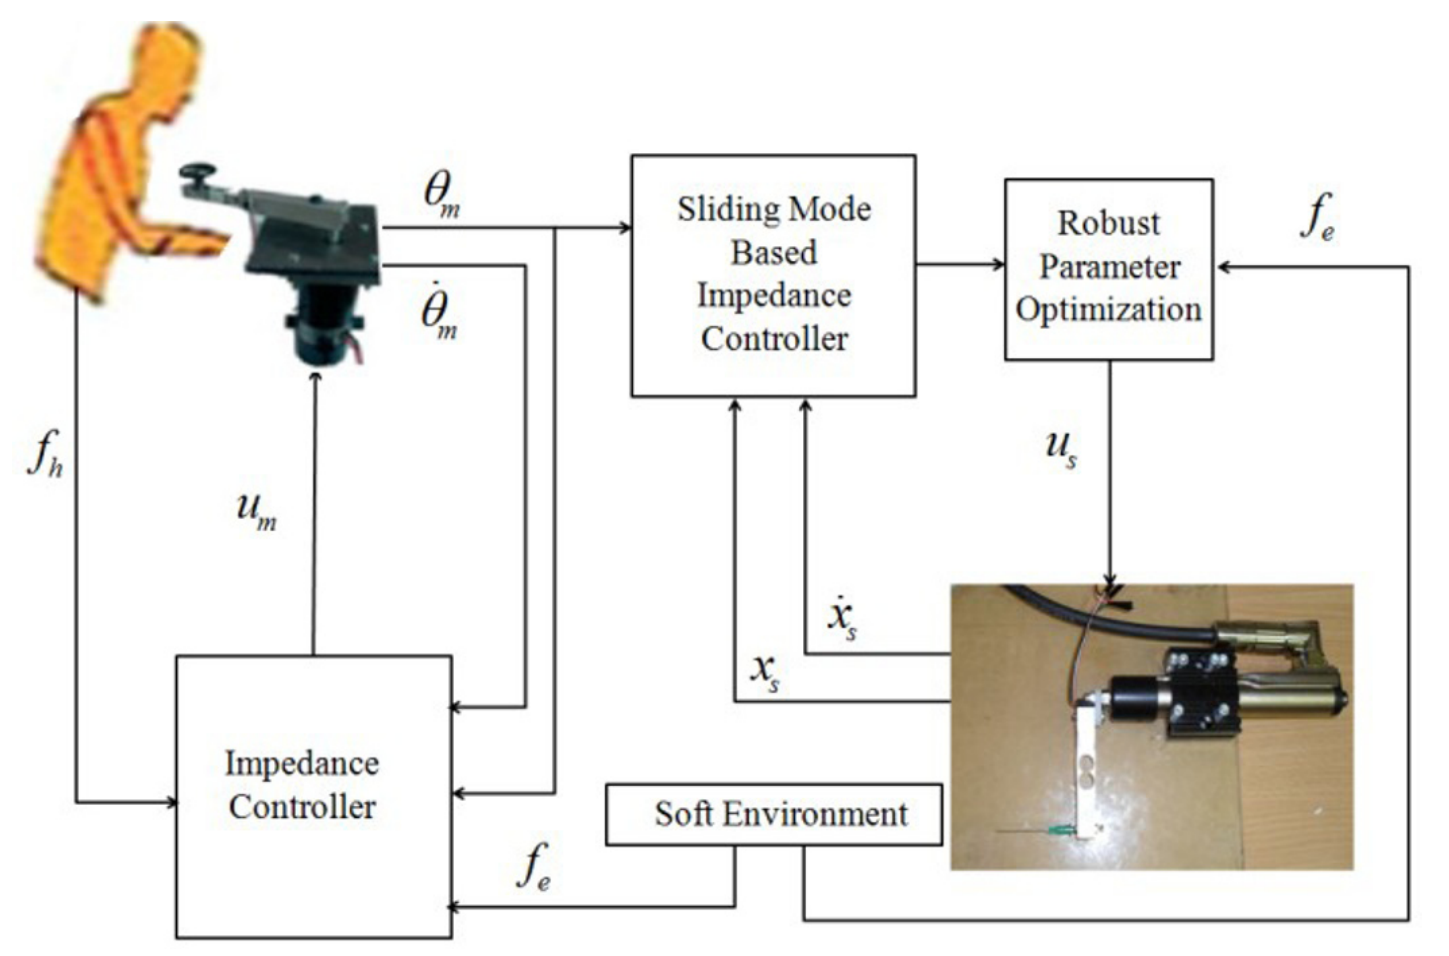
\includegraphics[width=\textwidth]{images/sliding_teleop.png}
	\caption[Haptic teleoperation schema (Dehghan)]{Dehghan teleoperation schema.  \cite{Dehghan2011}}
	\label{fig:sliding_teleop}
\end{figure}

The last work mentioned here is the one on wich this work is based. If falls both under the the umbrella of autonomous and teleoperated robots for needle insertion.
The work of Ferraguti \textit{et al.} \cite{Ferraguti2015} uses a variable admittance control on a custom developed stiff and not backdrivable robot to autonomously perform the punturing action.\\
In autonomous operation to reproduce the surgeon's behaviour, the chosen interaction model is a variable mass-spring-damper model. The possible loss of passivity of the controller due to the time-variable parameters has been addressed formulating the interaction model as a port-Hamiltonian system, endowed with an energy tank, in order to store the energy dissipated by the system and use it for a passive threatment of non passive behaviours like the variable admmitance.\\
When an intervetion of an operator is required, the system provides a safe way to switch to a teleoperated mode.
Here the coupling between master and slave is made by a virtual spring-damper, and the problem of initial decoupling between master and slave has been addressed with a time variable spring-like element which acts, for a limited amount of time, mainly on the master side to couple it to the slave without causing abrupt changes at slave side.

\section{Discussion}
Needle insertion is a complex procedure that involves a non-trivial effect, needle's bending, which is also non-trivial both to model an control.
When performing this action the clinician relays on kinestetic feedback and visual feedback. The former provides information on the moment of punturing and the tissiue tipe, the latter gives a feedback on the target and also on tissues type.
The needle bending could be exploited expecially by robotic procedures to provide a more precise target reaching and to avoid ostacle on the insertion path.

In order to design a fully automated system a precise model of the forces acting on the needle, a clear identification of punturing stages (pre, post andpuncturing) and a predictive model of tissue deformation are needed to develop control strategies and path plannig. The system also need a feedback that should provide needle and target tracking, and information on the environment like the interaction forces.
Engineering and integrating such a system is really challenging.
Becouse of the surgeon expertise with challenging task and unexpected situations the preffered clinical solution is to develop a robotic assited device that assists the operator in the positioning phase but demands to the clinician the insertion phase.

Telerobotics could be a valuable solution to put clinitian's expertise in the loop while enhancing the procedure's precision. However it has to deal with the classical teleoperation trade off between stability and transparency as we will discuss in the following chapter. In particular for the punturing action the main issue is the abrupt change in the force at the puncturing time which may induce in the operator an unwanted refletion feedback that breaks the transparency. 
%%%%%%%%%%%%%%%%%%%%%%%%%%%%%%%%%%%%


\clearpage
\thispagestyle{empty}